\section{Responsible Solution Design}
% 900 @ 866
\label{sec:responsible}
\begin{figure}[ht]
	\centering
	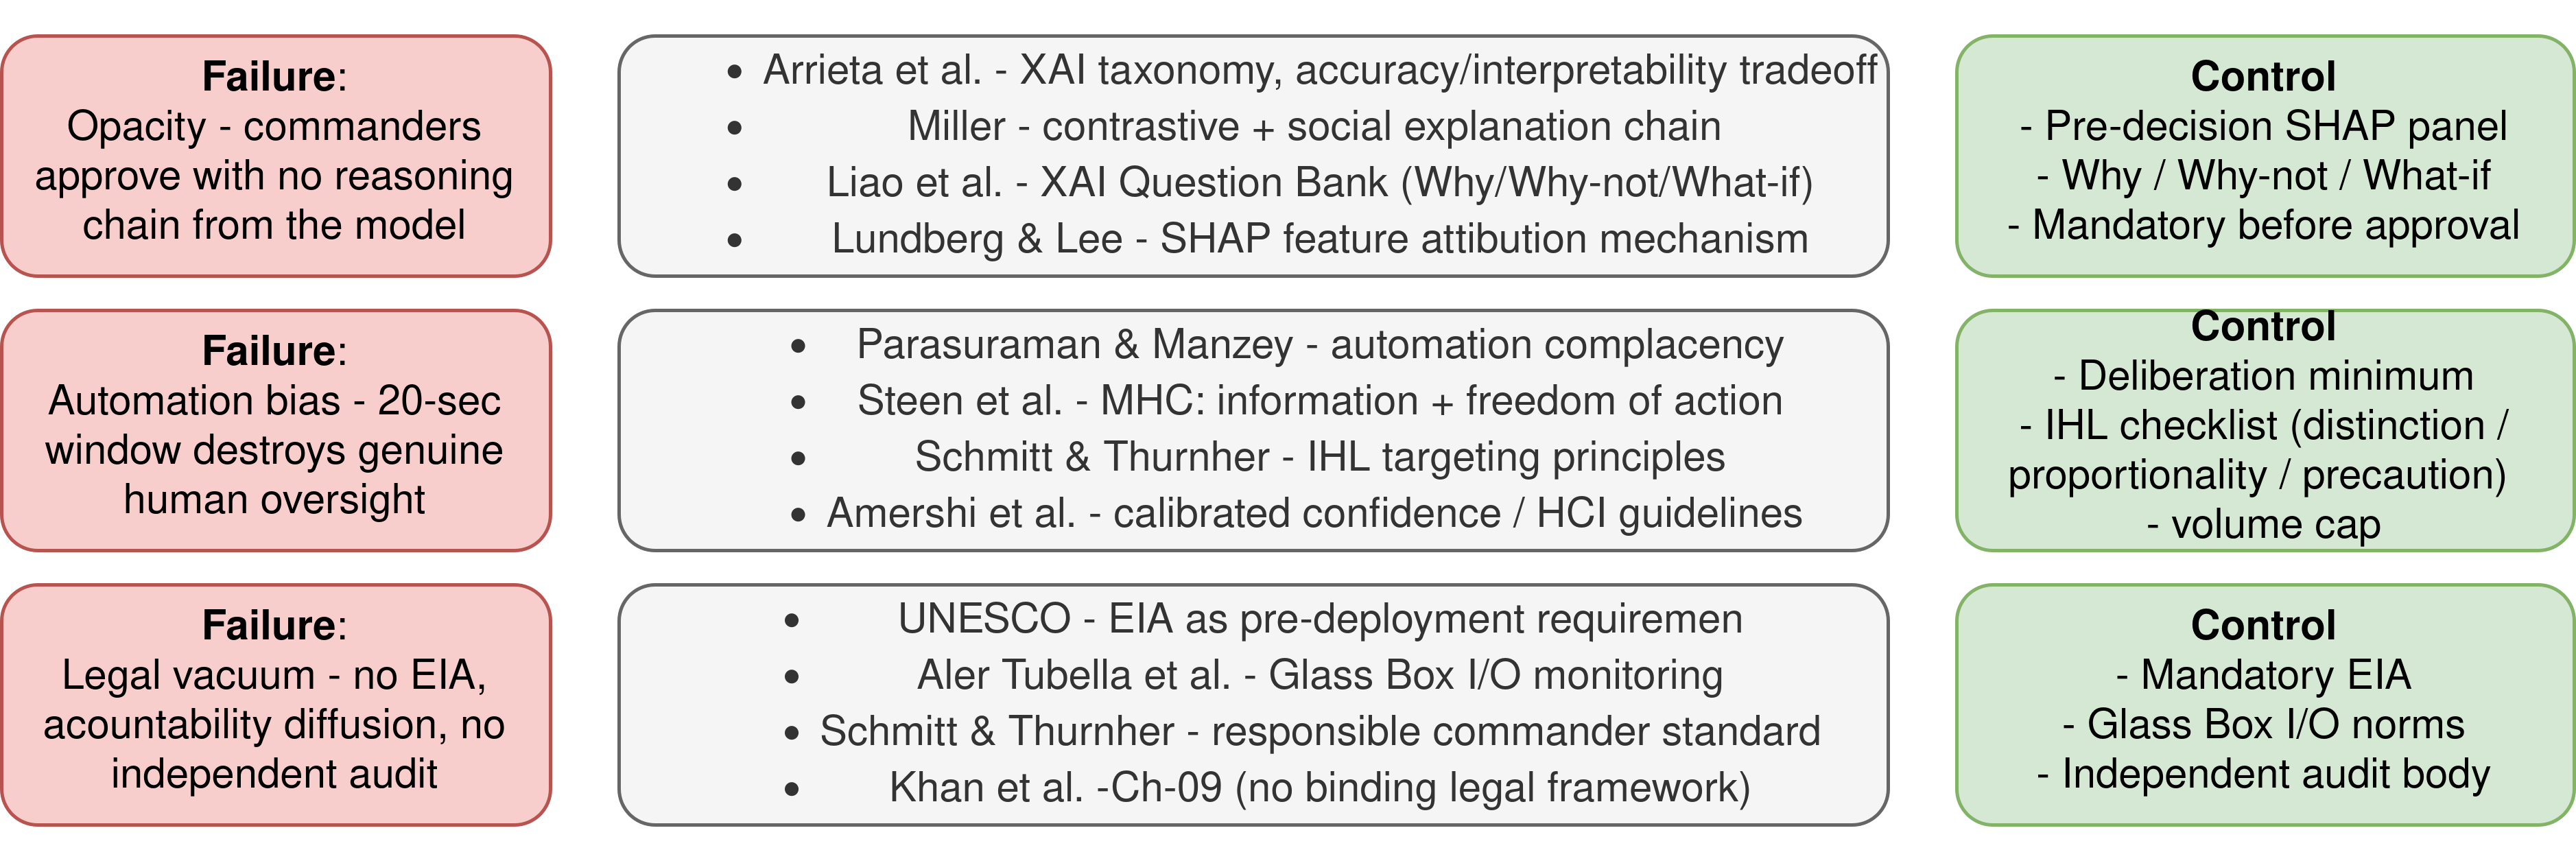
\includegraphics[width=0.8\textwidth]{images/Failures.drawio(1).png}
	\caption{Framework-to-solution map: each identified failure mode (left) linked to the diagnosing it (centre) and the proposed control (right).}
	\label{fig:failures}
\end{figure}
\subsection{Technical}
% Alexander
One technical failure identified in Section~\ref{sec:ethical} is that operators receive target recommendations without a reasoning chain. The direct remedy would be a transparency-by-design philosophy, but given that these models would trigger the accuracy/interpretability trade-off \citep{arrieta2019explainableartificialintelligencexai}, this adoption would be unlikely. A more realistic alternative would be implementing post-hoc explainability, integrated into the operators user interface. With this, as noted by \citet{arrieta2019explainableartificialintelligencexai}'s audience-centred definition: explainability is always relative to a given audience, the implementation should be calibrated to the field-operator, not for a Machine Learning engineer debugging the model weights.

%We propose two post-hoc interpretability methods, SHapley Additive exPlanations (SHAP) \cite{lundberg2017unifiedapproachinterpretingmodel} and Gradient-weighted Class Activation Mapping (Grad-CAM). SHAP assigns each input feature a contribution score for a prediction. For example a targetting recommendation for a building can be driven for 47\% by the targets movement patterns, for 30\% by their phone's metadata, and for 23\% by using drone footage showing targets entering it. Additionally, SHAP is model-agnostic and is therefore applicable to Habora's ensemble architecture, without accessing the models internals. Combined with Grad-CAM, which highlights images to show which parts contributed to the predictions (ref image), creates an evidential basis of each recommendation.
\label{sec:gradcam}
\begin{figure}[ht]
	\centering
	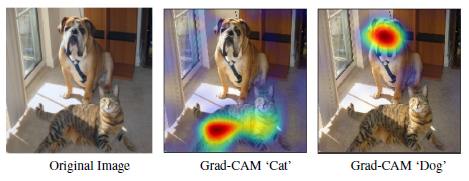
\includegraphics[width=0.8\textwidth]{images/modified-figure-1-dog-cat.png}
	\caption{Canonical Grad-CAM example \citep{gradcam}. Class heatmaps localise image regions for 'cat' and 'dog'. Applied to `Habsora', this method would highlight satellite or drone imagery for classification.}
	\label{fig:gradcam}
\end{figure}
We propose two post-hoc interpretability methods, SHapley Additive exPlanations (SHAP) \citep{lundberg2017unifiedapproachinterpretingmodel} and Gradient-weighted Class Activation Mapping (Grad-CAM Figure~\ref{fig:gradcam})\citep{gradcam}. SHAP assigns each input feature a contribution score for a prediction. For example, a targetting recommendation for a building can be driven for 47\% by the targets movement patterns, for 30\% by their phone's metadata, and for 23\% by using drone footage showing targets entering it. Being model-agnostic (such as KernelSHAP), it can be applied to Habsora's ensemble without accessing the models internals.

However, raw feature attribution is necessary but not sufficient. \citet{miller2018explanationartificialintelligenceinsights} identifies four properties of human explanation: they're contrastive (why X rather than Y), selective (not exhaustive), causal rather than probabilistic, and involve a social process between the explainer and explainee. SHAP's raw output does not satisfy any of these properties and must therefore be expanded upon by providing the operator with a contrastive explanation: not only recommending the 'best' target, but also presenting the nearest non-target alternative alongside its scores. This allows the operator to evaluate 'why this target rather than no strike', critically assess the recommendation, and override it if necessary.

\citet{liao2020questioning}'s XAI `QuestionBank' operationalises this further. From the ten categories in their taxonomy, three are decision-critical for a strike: `why', `why not' and `what if'. There align with \citet{miller2018explanationartificialintelligenceinsights}'s contrastive account (why X rather than Y) and map directly onto IHL's targeting principles: \textit{Why} supports distinction, \textit{Why not} supports proportionality, and \textit{What if} enables the precautionary assessment.
%Their taxonomy identifies questions which users need answered to make informed decisions: `why', `why not' and `what if'. These map directly into IHL requirements: \textit{Why} supports distinction, \textit{Why not} supports proportionality, and \textit{What if} enables the precautionary assessment. The design of the interface should have these as mandatory fields, not optional features. %\citet{morley2020what} note that post-hoc explainability tools tend to only be used at the testing stage of the ML-pipeline. Our recommendation insists that this should also be implemented in the operational deployment, not only during the systems validation. 
% Already in discussion

\subsection{Socio-technical}
% Alexander's stukje
As noted earlier, even if the technical layer would provide perfect explanations, the operational tempo would still undermine meaningful use. \citet{mhcof} define two conditions of moral responsibility: adequate information and meaningful freedom of action. Our proposed mechanism is a mandatory minimum deliberation time, with a hard interface lock. The operator cannot approve any strike before the review period has elapsed, ensuring that the deliberation standard is met by design, and preventing premature confirmation.

%\citet{aimag.v40i1.2848}'s LOAC compliance framework specifies what this deliberation standard must contain. Instead of a single button press approving the recommendation, the workflow should decompose this into confirmations aligned with IHL's core principles: \textit{distinction} (is this a valid military target?), \textit{proportionality} (is the anticipated military advantage proportionate to the expected civilian harm?), and \textit{precaution} (have all measures to minimise civilian harm been made?). For each question a separate confirmation must be given, which also serves as the legal standard as identified by \citet{ootlaws}, and prevents a multi-step legal judgement into a single button press.
The content of this deliberation follows IHL's targeting priciples, rather than a single button press, the workflow should decompose into separate confirmations: \textit{distinction} (is this a valid military target?), \textit{proportionality} (is the anticipated military advantage proportionate to the expected civilian harm?), and \textit{precaution} (have all measures to minimise civilian harm been made?). Requiring a confirmation per principle implements the legal standard identified by \citet{ootlaws}, and prevents a multi-step judgement into a single button press.

Moveover, \citet{parasuraman2010complacency} demonstrate that automation complacency is most pronounced when automation is highly and consistently reliable and when operators face competing task demands. The interface must actively interrupt this cycle by requiring engagements checks in the explanation layer: an operator should not be able to click through the IHL checklist without first reviewing the contrastive explanations and feature weights suggested before. This creates a forced interaction with the XAI output, counteracting that the explanation becomes a goal to be bypassed by the operator.
Expanding on this, \citet{amershi2019guidelines}'s human-AI interaction guidelines add it should: communicate how well the system can perform, calibrating displayed confidence to actual reliability, and uncertainty. Both directly countering the automation bias by insinuating trust.

% Harman's stukje no new content
%\citet{miller2018explanationartificialintelligenceinsights} reinforces the case for active engagement by specifying the types of questions an explanation must answer to be actionable: why a target was selected, why an alternative was not, and what would change under different inputs.

%Shortened
%The head-up display (HUD) for the operator could contain information, such as confidence, reliability and uncertainty, that makes the use of Habsora in that particular instance explainable. For example, the system can show a percentage likelihood that the strike will hit the right target. \citet{amershi2019guidelines}'s human-AI interaction guidelines, specify that systems must calibrate displayed confidence to actual reliability and communicate uncertainty explicitly. Each of these principles directly addresses the trust miscalibration that underlies automation bias.

% Shortened, removed speculation/limitation here
%\citet{friedman2013vsd}'s VSD methodology requires that indirect stakeholders' values are embedded in the system's design. Civilian presence in the target environment cannot remain pure metadata. Instead, value-laden indicators such as civilian density or protected-site proximity should be surfaced in the operator interface as a structural requirement. Considering the troublesome relationship between the Palestinians and the Israelis, such a process would likely require intermediary agents to facilitate the process, like the United Nations or another impartial international body.
Lastly, \citet{friedman2013vsd}'s VSD methodology requires that indirect stakeholders' values are embedded in the system's design. Civilian presence in the target environment cannot remain pure metadata: value-laden indicators such as civilian density or protected-site proximity should be surfaced in the operator interface as a structural requirement.

\subsection{Governance}
% Harman > nergens anders stahl gebruikt, kunnen verdiesen of wasilow/thorpe gebruiken
% \citet{stahl2022organisational}'s three-level mitigation typology provides a useful organising frame for the governance solutions we propose. Firstly, because it maps onto the temporal dimension of the CHOF matrix, making it clear where each intervention fits in the system lifecycle. And secondly, because it emphasises that policy-level strategies, guidance mechanisms, and corporate governance measures must be implemented together to effectively address the identified gaps in governance.

Governance interventions must be staged across the whole lifecycle of the systems, as reflected in the temporal axis of the CHOF \citep{info12090385} and the staged ethics-assessment approach advocated by \citet{aimag.v40i1.2848}.

\subsubsection{Pre-deployment} %Shortened
%A mandatory pre-deployment ethical impact assessment (EIA) should be grounded in UNESCO's recommendation against delegating life-or-death decisions to AI~\citep{unesco2021recommendation}. This would ensure that human rights implications are systematically reviewed before deployment. Voluntary review processes, like Canada's legal assessment protocol~\citep{aimag.v40i1.2848}, would be insufficient. Binding policy-level requirements are necessary to prevent the kind of gaps in governance we see in Israel's non-ratification of Protocol I to the Geneva Conventions. This gap can be categorised using \citet{khan2021ethicsaisystematicliterature}'s CH-09: the absence of institutionalised ethical review mechanisms in AI deployment.
A mandatory pre-deployment ethical impact assessment (EIA) should be grounded in UNESCO's recommendation against delegating life-or-death decisions to AI~\citep{unesco2021recommendation}. Ensuring that human rights implications are systematically reviewed before deployment. Binding policy-level requirements are necessary to prevent the kind of gaps in governance addressing the gaps identified in \citet{khan2021ethicsaisystematicliterature}'s \textbf{P-03} accountability and \textbf{P-05} autonomy, regarding the absence of accountability mechanisms and the erosion of human agency in AI systems.
%we see in Israel's non-ratification of Protocol I, as categorized by \citet{khan2021ethicsaisystematicliterature} as CH-09: the absence of institutionalised ethical review mechanisms.

\subsubsection{During deployment}
Glass Box compliance norms~\citep{ijcai2019p802} should be followed during deployment: documented input/output thresholds for the system's recommendations, mandatory escalation criteria for when human operators must intervene, and post-strike logs recording which recommendation was authorised and on what basis. %According to \citet{info12090385}, this should not remain an optional design choice, but rather an operational legal requirement.
\citet{info12090385} integrate this appreoad into the governance layer of the CHOF: we argue it should not remain an optional design choice, but rather an operational legal requirement.

\begin{figure}[ht]
	\centering
	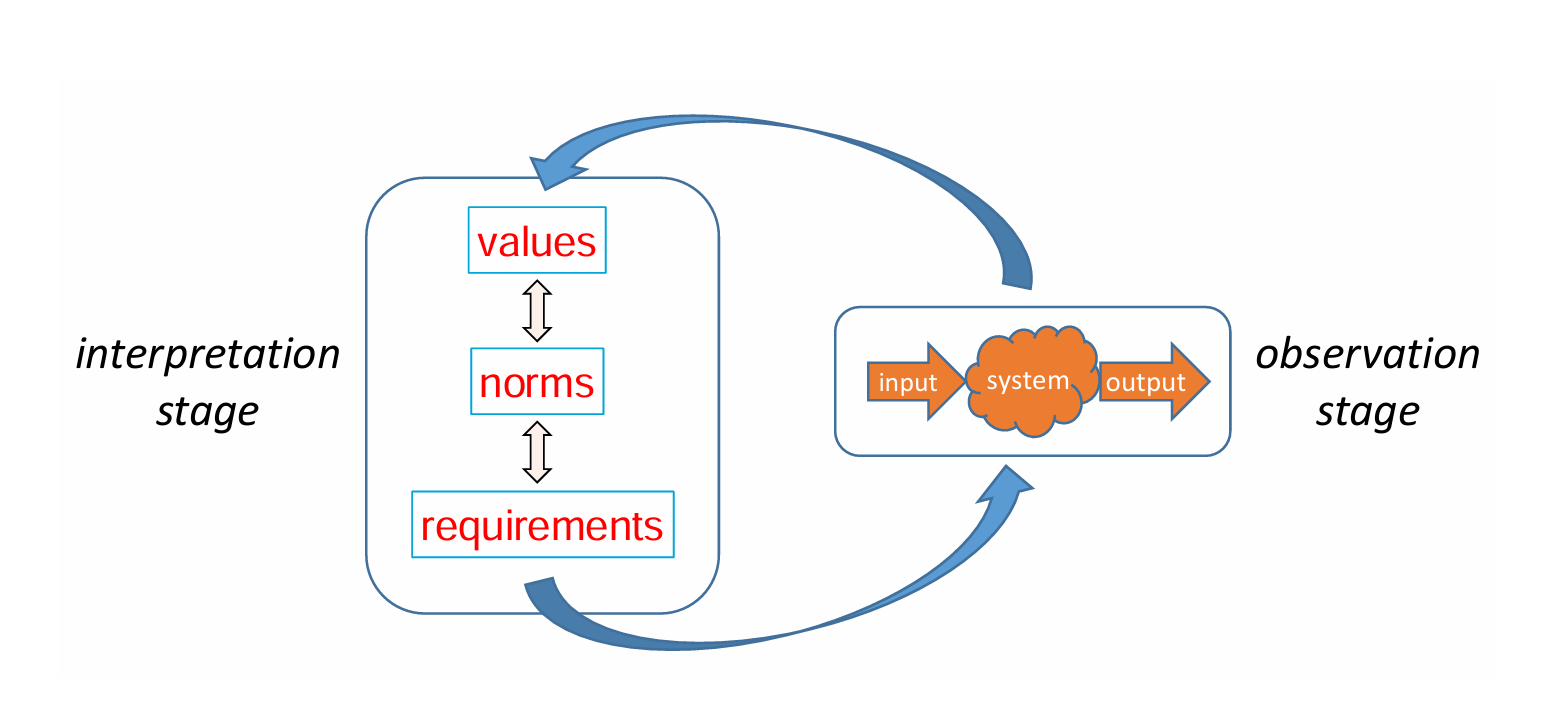
\includegraphics[width=0.8\textwidth]{images/GlassBox.png}
	\caption{The Glass Box approach translates abstract values, such as human dignity, into observable norms and requirements to be implemented in the the AI system~\citep{info12090385, ijcai2019p802}}
\end{figure}

\subsubsection{Post-deployment}
An independent auditor should have access to the Glass Box logs to verify compliance with International Humanitarian Law and identify any violations. This would address the responsibility diffusion problem by replacing it with a traceable chain of authorisation, consistent with the responsible-operator standard set out by \citet{ootlaws}. This would restore accountability and the possibility of redress for affected parties, addressing the gaps identified in \citet{khan2021ethicsaisystematicliterature}'s \textbf{P-01} transparency and \textbf{P-03} accountability: the audit trail makes the authorisation chain inspectable and traceable.

%None of these levels of governance intervention is sufficient on their own. The CHOF matrix makes this explicit by showing how the absence of governance measures at each stage of the system lifecycle creates gaps that can be exploited.


% Total: intro + rsd 1300/1250
% Todo: images (3) + text, British English, proofread, verify sources.